\section{Gleichungen in \texorpdfstring{$\C$}{C}}
\subsection{Lineare Gleichungen}
Lineare Gleichung können in $\C$ genau gleich wie in $\R$ gelöst werden.

\begin{bsp}
    {Lineare Gleichung in $\C$}{}

    $$ 2i+z = 5z -3 + iz$$

    \vspace*{7cm}
    

\end{bsp}

\begin{ueb}
{}{}
\begin{enumerate}
    \item Löse folgende Gleichungen und stelle die Lösung in Normalform dar.
    \begin{enumerate}
        \item $5z = 8iz + (81 - 5i)$
        \item $(2 - i)z + i = 2 + z$
        % \item $z = \frac{3z + i}{2 - 2i}$
        % \item $z - i(4 + z) = 3(z - 2) + 5i$
        % \item $z(2 - 2i) = 3z + i$
        % \item $3z + 9i = iz - 4$
        \item $i(i + z) - (5 + 2i) = i(i - z) + 8$
        % \item $3i = \frac{7 - 2i - z}{z + 4 + 3i}$
    \end{enumerate}

    \item In den folgenden Gleichungen kommen $z$ und die zu $z$ konjugiert komplexe Variable $\bar{z}$ vor. Setze $z = x + iy$ und löse anschliessend ein reelles Gleichungssystem für $x$ und $y$.
    \begin{enumerate}
        \item $z + 2i \bar{z} = 8 + 7i$
        \item $2z - i \bar{z} = 1$
        \item $\frac{\bar{z} + i}{z - i} = 1$
        %\item $4z^2 - 4\bar{z} + 1 = 0$
        
        % \item $z + 2 \bar{z} = 3 - i$
        %\item $(1 + i)z + (1 - i)\bar{z} = 1$
    \end{enumerate}
\end{enumerate}
\end{ueb}
\clearpage
\emph{Lösungen}
\begin{enumerate}
 
\item Lösungen der Gleichungen:
\begin{enumerate}
    \item $5 + 7i$
    \item $\frac{3}{2} + \frac{1}{2}i$
    % \item $-\frac{2}{5} - \frac{1}{5}i$
    % \item $\frac{3}{5} - \frac{24}{5}i$
    % \item $-\frac{2}{5} - \frac{1}{5}i$
    % \item $-\frac{3}{10} - \frac{31}{10}i$
    \item $1 - \frac{13}{2}i$
    % \item $-\frac{13}{5} - \frac{31}{5}i$
\end{enumerate}

\item Lösungen:
\begin{enumerate}
    \item $2 + 3i$
    \item $\frac{2}{3} + \frac{1}{3}i$
    \item $t + i, \text{ wobei } t \in \mathbb{R}^* \text{ beliebig}$
   % \item $\frac{1}{2}, -\frac{1}{2} + i, -\frac{1}{2} - i$
   
    % \item $1 + i$
    %\item $\frac{1}{2} + t(1 + i), \text{ wobei } t \in \mathbb{R} \text{ beliebig}$
\end{enumerate}
\end{enumerate}
















\clearpage
\subsection{Gleichungen der Form \texorpdfstring{$z^n = c$}{z**n=c}}
\begin{LA}
    {}{}
    In dieser Aufgabe sollen die Lösungen der Gleichung 
    $$z^2=4i$$
    ermittelt werden.
    Gehen Sie dafür wie folgt vor.
    \begin{enumerate}
        \item Schreiben Sie die beiden Seiten der Gleichung in Polarform. Das heisst: Setzen Sie $z=r\cdot \cis(\varphi)$, was ist dann $z^2$? Wie lautet die Polarform von 4i?
        \item Vergleichen Sie Betrag und Argument der Polarform auf der linken mit jenen der rechten Seite der Gleichung. Können Sie damit eine Lösung der Gleichung finden?
        
        (Kontrolle: sie lautet $z_1=\sqrt{2}+\sqrt{2}i$)
        \item Die Gleichung hat eine weitere Lösung $z_2$ mit dem gleichen Betrag wie $z_1$, aber einem anderen Argument. Können Sie die zweite Lösung erraten? 
    \end{enumerate}


%     \begin{center}
%     \begin{tikzpicture}[scale = 0.7]
%         % Gitter
%         \draw[dashed, very thin, gray] (-5,-5) grid (5,5);
        
%         % Achsen mit Skala
%         \draw[->] (-5,0) -- (5,0) node[above] {$\RE$};
%         \draw[->] (0,-5) -- (0,5) node[right] {$\IM$};
%         \foreach \x in {-4,-3,-2,-1,1,2,3,4} 
%             \draw (\x,0) -- (\x,-0.2) ;
%          \foreach \y in {-4,-3,-2, -1,2,3,4}
%             \draw (0,\y) -- (-0.2,\y) ;
%         \draw (0,1) -- (-0.2,1) node[left] {$i$};
%         \draw (1,0) -- (1,-0.2) node[below] {$1$};
        
%         % Punkte und Markierungen
%         %\draw[dashed] (0,0) circle (4);
%         \fill[blue] (0,4) circle (0.05) node[above right, blue] {$4i$};
%     \end{tikzpicture}
% \end{center}
\end{LA}




\clearpage
\begin{bsp}
    {Lösungen von $z^6=64$}{}
    Gegeben ist die Gleichung
    $$z^6=64$$



    \vspace*{20cm}





\end{bsp}

\clearpage
\begin{satz}
    {Lösungen der Gleichung $z^n=c$}{}
    Die Gleichung $z^n = r\ \cis(\varphi)$ hat die $n$ Lösungen:
    \[ z_k = \sqrt[n]{r} \operatorname{cis} \left( \frac{\varphi + 2\pi k}{n} \right), \quad k = 0, 1, \dots, n-1. \]
    Die Lösungen befinden sich alle auf einem Kreis mit Radius $\sqrt[n]{r}$. Sie bilden die Ecken eines regelmässigen $n$-Ecks.

   
\end{satz}

\begin{bsp}
    {}{}
    Das folgende Bild zeigt die fünf Lösungen der Gleichung 
    $$z^5=40+40i$$
    \begin{center}

        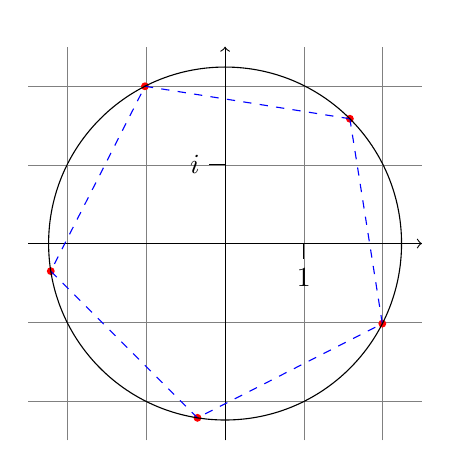
\begin{tikzpicture}
            \draw[very thin, gray] (-2.5,-2.5) grid (2.5,2.5);
            \draw[->] (-2.5,0) -- (2.5,0) node[right] {$\RE$};
            \draw[->] (0,-2.5) -- (0,2.5) node[above] {$\IM$};
            \draw (0,1) -- (-0.2,1) node[left] {$i$};
            \draw (1,0) -- (1,-0.2) node[below] {$1$};
            
            % Radius berechnen
            \def\r{(40*sqrt(2))^(1/5)}
            \def\angle{atan(1)} % Argument von 1+i
            
            % Punkte speichern
            \coordinate (P0) at ({\r*cos((\angle+360*0/5))}, {\r*sin((\angle+360*0/5))});
            \coordinate (P1) at ({\r*cos((\angle+360*1/5))}, {\r*sin((\angle+360*1/5))});
            \coordinate (P2) at ({\r*cos((\angle+360*2/5))}, {\r*sin((\angle+360*2/5))});
            \coordinate (P3) at ({\r*cos((\angle+360*3/5))}, {\r*sin((\angle+360*3/5))});
            \coordinate (P4) at ({\r*cos((\angle+360*4/5))}, {\r*sin((\angle+360*4/5))});
            
            % Punkte einzeichnen
            \foreach \p in {P0, P1, P2, P3, P4} {
                \fill[red] (\p) circle (0.05);
            }
            
            % Fünfeck zeichnen
            \draw[dashed, blue] (P0) -- (P1) -- (P2) -- (P3) -- (P4) -- cycle;
            
            % Kreis zeichnen
            \draw[thin] (0,0) circle[radius=\r];
        \end{tikzpicture}

    \end{center}
\end{bsp}

\clearpage
\begin{ueb}{}{}
    \begin{enumerate}
        \item Finde alle Lösungen der Gleichungen:
        \begin{enumerate}
            \item $z^4 = 1$
            \item $z^5 = 1024i$
            %\item $z^6 = 64 \operatorname{cis} \left(\frac{\pi}{5}\right)$
            \item $z^3 = -2 + 2i$
        \end{enumerate}
        
        % \item Bestimme die Lösungen:
        % \begin{enumerate}
            
        %     \item $z^6 - \sqrt{3} = i$
        %     \item $z^6 = \left(\operatorname{cis} \left(\frac{\pi}{4}\right)\right)^4$
            
        % \end{enumerate}
        % \item Gegeben ist $z_0 = \sqrt{3} - i$ als eine Lösung der Gleichung $z^4 = a$. Berechne $a$ und die übrigen Lösungen.

        \item Die Skizze zeigt eine Lösung $z$ der Gleichung $z^4 = a$. Zeichne alle anderen Lösungen der Gleichung in die Zahlenebene.

        \begin{center}

            \begin{tikzpicture}
                \draw[very thin, gray] (-2.5,-2.5) grid (2.5,2.5);
                \draw[->] (-2.5,0) -- (2.5,0) node[right] {$\RE$};
                \draw[->] (0,-2.5) -- (0,2.5) node[above] {$\IM$};
                \draw (0,1) -- (-0.2,1) node[left] {$i$};
                \draw (1,0) -- (1,-0.2) node[below] {$1$};
                
                % Radius berechnen
                \def\r{1.5}
                \def\angle{60} 
                
                % Punkte speichern
                \coordinate (P0) at ({\r*cos((\angle+360*0/4))}, {\r*sin((\angle+360*0/4))});
                \coordinate (P1) at ({\r*cos((\angle+360*1/4))}, {\r*sin((\angle+360*1/4))});
                \coordinate (P2) at ({\r*cos((\angle+360*2/4))}, {\r*sin((\angle+360*2/4))});
                \coordinate (P3) at ({\r*cos((\angle+360*3/4))}, {\r*sin((\angle+360*3/4))});
               
                
                % Punkte einzeichnen
                % \foreach \p in {P0, P1, P2, P3, P4} {
                %     \fill[red] (\p) circle (0.05);
                % }
                \fill[red] (P0) circle (0.05);



                % Fünfeck zeichnen
                %\draw[dashed, blue] (P0) -- (P1) -- (P2) -- (P3) -- (P4) -- cycle;
                
                % Kreis zeichnen
                %\draw[thin] (0,0) circle[radius=\r];
            \end{tikzpicture}
    
        \end{center}

        \item Die Gleichungen der Form $z^n = 1$ heissen Kreisteilungsgleichungen. Die Lösungen solcher Gleichungen heissen \textit{$n$-te Einheitswurzeln}.
        \begin{enumerate}
           
            \item Berechne die Summe aller 6. Einheitswurzeln. Verallgemeinerung?
            \item  Berechne das Produkt aller 5. Einheitswurzeln. Verallgemeinerung?
        \end{enumerate}
    \end{enumerate}
\end{ueb}

\clearpage
\emph{Lösungen}
\begin{enumerate}
    \item Lösungen der Gleichungen:
    \begin{enumerate}
        \item \( z^4 = 1 \Rightarrow z \in \{1, i, -1, -i\} \)
        \item \( z^5 = i \Rightarrow z_k = 4\operatorname{cis} \left( \frac{\pi}{10} + \frac{2k\pi}{5} \right), k = 0,1,2,3,4 \)
        %\item \( z^6 = 64 \operatorname{cis} \left(\frac{\pi}{5}\right) \Rightarrow z_k = 2 \operatorname{cis} \left( \frac{\pi}{30} + \frac{2k\pi}{6} \right), k = 0,1,2,3,4,5 \)
         \item \( z^3 = -2 + 2i \Rightarrow z_k = \sqrt{2} \operatorname{cis} \left( \frac{\pi}{4} + \frac{2k\pi}{3} \right), k = 0,1,2 \)
    \end{enumerate}

    \item Lösungen zeichnen
    
    \begin{center}

        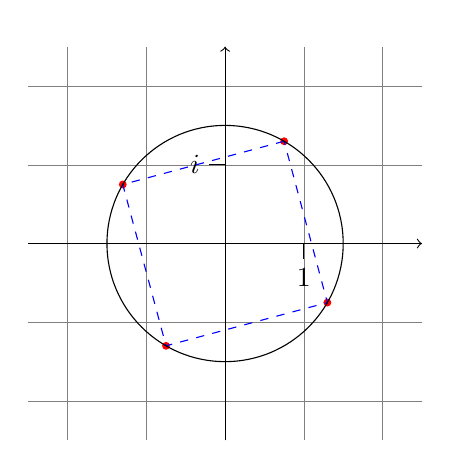
\begin{tikzpicture}
            \draw[very thin, gray] (-2.5,-2.5) grid (2.5,2.5);
            \draw[->] (-2.5,0) -- (2.5,0) node[right] {$\RE$};
            \draw[->] (0,-2.5) -- (0,2.5) node[above] {$\IM$};
            \draw (0,1) -- (-0.2,1) node[left] {$i$};
            \draw (1,0) -- (1,-0.2) node[below] {$1$};
            
            % Radius berechnen
            \def\r{1.5}
            \def\angle{60} 
            
            % Punkte speichern
            \coordinate (P0) at ({\r*cos((\angle+360*0/4))}, {\r*sin((\angle+360*0/4))});
            \coordinate (P1) at ({\r*cos((\angle+360*1/4))}, {\r*sin((\angle+360*1/4))});
            \coordinate (P2) at ({\r*cos((\angle+360*2/4))}, {\r*sin((\angle+360*2/4))});
            \coordinate (P3) at ({\r*cos((\angle+360*3/4))}, {\r*sin((\angle+360*3/4))});
           
            
            % Punkte einzeichnen
            \foreach \p in {P0, P1, P2, P3} {
                \fill[red] (\p) circle (0.05);
            }
            %\fill[red] (P0) circle (0.05);



            % Viereck zeichnen
            \draw[dashed, blue] (P0) -- (P1) -- (P2) -- (P3) -- cycle;
            
            % Kreis zeichnen
            \draw[thin] (0,0) circle[radius=\r];
        \end{tikzpicture}

    \end{center}

    % \item Lösungen der Gleichungen:
    % \begin{enumerate}
       
    %     \item \( z^6 - \sqrt{3} = i \Rightarrow z_k = \sqrt[6]{2}\operatorname{cis} \left( \frac{\pi}{36} + \frac{2k\pi}{6} \right), k = 0,1,2,3,4,5 \)
    %     \item \( z^6 = \left(\operatorname{cis} \frac{\pi}{4}\right)^4 \Rightarrow z_k = \operatorname{cis} \left( \frac{\pi}{6} + \frac{2k\pi}{6} \right), k = 0,1,2,3,4,5 \)
        
    % \end{enumerate}
    % \item \( a = 16\cis(\frac{4\pi}{3}), \) übrige Lösungen: \( z_k = 2 \operatorname{cis} \left( \frac{\pi}{3} + \frac{2k\pi}{4} \right), k = 0,1,2,3 \)

    \item Kreisteilungsgleichungen:
    \begin{enumerate}
 
        \item Summe aller 6. Einheitswurzeln: \( 0 \). Verallgemeinerung: Die Summe aller \( n \)-ten Einheitswurzeln ist \( 0 \), falls \( n > 1 \) gerade. (Das stimmt auch für ungerade $n$, was man mit dem Fundamentalsatz der Algebra zeigen kann (weiter unten))
        \item Produkt aller 5. Einheitswurzeln: \(  1 \). Verallgemeinerung: Das Produkt aller \( n \)-ten Einheitswurzeln ist \( \cis\left(\frac{2\pi}{n} (1+2+3+\cdots n)\right)= \cis((n+1)\pi) = \left(\cis (\pi)\right)^{n+1} = (-1)^{n+1} \).    \end{enumerate}
\end{enumerate}



















\clearpage
\subsection{Quadratische Gleichungen}
Die Lösungsformel für quadratische Gleichungen in $\R$ bleibt mit kleinen Anpassungen auch für quadratische Gleichungen in $\C$ gültig:

\begin{satz}
    {Quadratische Gleichung mit reellen Koeffizienten}{}
    Für eine quadratische Gleichung der Form $az^2+bz+c=0$ mit $a,b,c\in\R$ gilt:

    Ist die Diskriminante $D=b^2-4ac \ge0$, so gilt die bekannte Auflösungsformel.

    Ist die Diskriminante $D=b^2-4ac <0$, so sind die Lösungen:
    $$z_{1,2} = \frac{-b\pm \sqrt{|D|}i}{2a}$$
\end{satz}

\begin{bsp}
    {Quadratische Gleichung mit reellen Koeffizienten}{}
    $$z^2+2z+2=0$$

    \vspace*{3cm}

\end{bsp}

Der Satz scheint auf den ersten Blick etwas umständlich formuliert. Das liegt daran, dass man streng genommen keine Wurzel von negativen Zahlen verwenden darf, weil diese nicht restlos definiert werden kann (welches ist die Wurzel von $-1$? Ist es $i$ oder $-i$?). Wegen des $\pm$ vor der Wurzel in der Auflösungsformel besteht hier aber keine Gefahr, dass durch die Verwendung der Wurzel Widersprüche entstehen. 


Die gleiche Formel gilt im Wesentlichen auch für quadratische Gleichungen, wenn die vorkommenden Koeffizienten komplex sind. 
\begin{satz}
    {Quadratische Gleichung mit komplexen Koeffizienten}{}
    Für eine quadratische Gleichung der Form $az^2+bz+c=0$ mit $a,b,c\in\C$ gilt:

    $$z_{1,2} = \frac{-b\pm w}{2a}$$
    Wobei $w$ die Lösung der Gleichung $w^2=D=b^2-4ac$ ist.
\end{satz}

Auch hier ist die Formulierung auf den ersten Blick nicht ganz einfach, weil es keine eindeutige Wurzel von komplexen Zahlen gibt. In der Praxis (Siehe \Cref{bsp:QuGlKomplex} ) wird das Problem der Doppeldeutigkeit durch das $\pm$ wieder entschärft.

\pagebreak
\begin{bsp}
    {Quadratische Gleichung mit komplexen Koeffizienten}{QuGlKomplex}
    \[
z^2 + (5 - 7i)z - 12 - 20i = 0
\]


\vspace*{20cm}

\end{bsp}

\clearpage
\begin{ueb}
    {}{}
    \begin{enumerate}
        \item \begin{enumerate}
            \item\( z^2 - 6z + 13 = 0 \)
            \item \( z^2 + z + 1 = 0 \)
            \item \( z^2 (2 + z^2) = 15 \)
            % \item \( 4z^2 + 8z + 5 = 0 \)
             \item \( \frac{4}{5}z - \frac{1}{5}z^2 = -9 \)
            % \item \( z^4 + 4z^2 + 3 = 0 \)
            % \item \( 2z^2 + 2z + 5 = 0 \)
            \item \( z^5 - 2z^4 + 2z^3 = 0 \)
        \end{enumerate}
        \item Begründen Sie die folgende Aussage: Wenn $z$ die Lösung einer quadratischen Gleichung mit reellen Koeffizienten ist, so ist auch $\bar z$ eine Lösung der Gleichung.
        \item \begin{enumerate}
            \item \( z^2 - iz + i = z \)
            \item \( 4z(z - 2i) - 3 = 5(z - i) \)
            \item \( z^2 - 2iz = 1 + 8i \)
            \item   \( z^2 + iz + 3i + 1 = 0 \)
        \item \( 1 - \frac{2i}{z} = iz \)
        \end{enumerate}
        
    \end{enumerate}
\end{ueb}

\clearpage
\emph{Lösungen}
\begin{enumerate}
    \item \begin{enumerate}
        \item \( 3 \pm 2i \)
        \item \( -\frac{1}{2} \pm \frac{\sqrt{3}}{2} i \)
        \item \( \pm \sqrt{3}, \pm \sqrt{5} i \)
        \item $-5, 9$
        \item \( 0, 1 \pm i \)
    \end{enumerate}
    \item \dots%Wenn die $z$ reell ist, ist $\bar{z}=z$ und damit auch eine Lösung. Wenn $z$ nicht reell ist. 
    \item 
        \begin{enumerate}
            \item \( 1, i \)
            \item \( 1 + i, \frac{1}{4} + i \)
            \item \( 2 + 3i, -2 - i \)
            \item \( 1 - 2i, -1 + i \)
            \item $i, -2i$
        \end{enumerate}
    
    
\end{enumerate}
























\clearpage
\subsection{Nullstellen von Polynome und der Fundamentalsatz}
\begin{definition}
    {Polynom}{}
    Ein Term der Form
\[
p(z) = a_n z^n + a_{n-1} z^{n-1} + \dots + a_1 z + a_0
\]
nennen wir ein \textbf{Polynom}.

Der \textbf{Grad} eines Polynoms ist die höchste vorkommende Potenz der Variable \( z \).

Die Zahlen \( a_0, a_1, a_2, \dots, a_n \) nennt man \textbf{Koeffizienten}.

Wenn alle Koeffizienten reell sind, so nennt man \( p(z) \) ein \textbf{reelles Polynom}.

\end{definition}

Eine wichtige Frage im Zusammenhang mit Polynomen ist, ob es bestimmte Zahlen \( z \) gibt, die eingesetzt in das Polynom den Wert 0 ergeben.
\begin{definition}
    {Nullstelle}{}

    Sei \( p(z) \) ein Polynom. Eine Nullstelle von \( p(z) \) ist eine Zahl \( z_0 \) mit der Eigenschaft, dass \( p(z_0) = 0 \) ist.

\end{definition}

\begin{bsp}
    {}{}
    \begin{enumerate}
        \item $
p_1(z) = z + 3
$
\vspace{2cm}

\item $
p_2(z) = z^2 - 4z + 5
$
\vspace{3cm}
\item $
p_3(z) = z^3 + 1$
\vspace{3cm}

    \end{enumerate}
\end{bsp}
\textbf{Bemerkung:} Um die Nullstellen eines Polynoms $n$-ten Grades zu ermitteln, muss man eine Gleichung $n$-ten Grades lösen.

\begin{bsp}
    {}{}
    Nullstellen des Polynoms:
\[
p(z) = z^3 + 5z^2 + 6z
\]

\vspace*{3cm}
\end{bsp}




\begin{definition}
    {Linearfaktor}{}
    Ein Term der Form $(z-z_0)$ heisst Linearfaktor.

\end{definition}
\begin{satz}
    {Linearfaktor $\leftrightarrow$ Nullstelle}{}
    Eine Zahl $z_0$ ist genau dann eine Nullstelle eines Polynoms $n$-ten Grades $p(z)$, wenn 

\[
p(z) = (z - z_0) \cdot q(z)
\]

wobei $q(z)$ ein Polynom vom Grad $n-1$ ist.

Man sagt, dass sich der Linearfaktor $(z - z_0)$ \emph{abspalten} lässt.
\end{satz}

\begin{definition}
    {Vielfachheit einer Nullstelle}{}
    Wenn sich der Linearfaktor $(z-z_0 )$ insgesamt $k$-mal vom Polynom $p(z)$ abspalten lässt, so nennt man $z_0$ eine $k$-fache Nullstelle oder eine Nullstelle mit Vielfachheit $k$ von $p(z)$.
\end{definition}
\begin{bsp}
    {Vielfachheiten}{}
    \begin{enumerate}
        \item $	(z-2) (z+3)^3 (z-2+i)$
         \vspace{2cm}
        \item $(z^2+1)(z^2+2z+1)(z^2-1)$
        \vspace{5cm}

    \end{enumerate}
\end{bsp}

%\subsection*{Der Fundamentalsatz der Algebra}

Dieser Fundamentalsatz der Algebra ist von grosser Bedeutung in der Mathematik. Den ersten vollständigen Beweis lieferte Carl Friedrich Gauss in seiner Dissertation (1799). Leider übersteigt der Beweis unsere Möglichkeiten. Aber mit den gelernten Begriffen können wir den Satz verstehen. 

\begin{satz}
    {Fundamentalsatz der Algebra}{}
    Ein Polynom $n$-ten Grades lässt sich in $\C$ in das Produkt von genau $n$ Linearfaktoren zerlegen.

    \bigskip

    In anderen Worten:

    \bigskip


    Ein Polynom $n$-ten Grades hat in der Grundmenge $\C$ genau $n$ Nullstellen (Vielfachheiten miteinberechnet) 

    \bigskip


    oder in einer dritten Variante:

    \bigskip

    Eine Gleichung $n$-ten Grades hat in der Grundmenge $\C$ genau $n$ Lösungen (Vielfachheiten miteinberechnet)

\end{satz}


\begin{bsp}
    {}{}

    
$$z^3-z^2+z-1=(z-1)(z-i)(z+i) $$
$$z^2+2iz-1=(z+i)(z+i) $$

\end{bsp}

\begin{ueb}
    {}{}
    \begin{enumerate}

        \item Bestimmen Sie die Nullstellen und deren Vielfachheiten:
        \[
        p(z) = (z^2 + 8z + 15)(z^2 - 25)(z^2 + 100)
        \]
    
        \item Zerlege das Polynom \( p(z) = z^5 - z^2 \) in ein Produkt von 5 Linearfaktoren.
    
        % \item Sei \( p(z) = z^7 - 42 \) und \( q(z) = 3z^4 + 2z^3 + z \).
        % \begin{enumerate}
        %     \item Welchen Grad haben \( p(z) - q(z) \) und \( p(z) \cdot q(z) \)?
        %     \item Beweisen Sie: Ein Polynom \( n \)-ten Grades kann höchstens \( n \) Nullstellen haben.
        % \end{enumerate}
    
       
    
        % \item \textbf{(Challenge)} Beweisen Sie: Das Produkt aller \( n \)-ten Einheitswurzeln ist \( (-1)^{n+1} \).
    \end{enumerate}
\end{ueb}

\clearpage
\emph{Lösungen}
\begin{enumerate}
    \item 
        $$z_1=-3, z_{2,3}=-5 \text{ zweifach } , z_4=5  ,  z_5 = 10i, z_6=-10i $$
    \item $$ p(z) = z^5 - z^2= z\cdot z \cdot\left(z-\cis\left(\frac{2\pi}{3}\right)\right)\cdot(z-1)\cdot\left(z-\cis\left(-\frac{2\pi}{3}\right)\right)$$ 

  
\end{enumerate}
